\chapter{Stéganographie}
\label{chap:BDD}

\section{Steghide}
\subsection{Définition}

Steghide est un programme de stéganographie permettant de masquer des données dans des fichiers image et audio. Il présente plusieurs fonctionnalités :\\
-        Compression des données incorporées.\\
-        Cryptage des données incorporées.\\
-        Incorporation d’une somme de contrôle pour vérifier l’intégrité des données extraites.\\
-        Prise en charge des fichiers JPEG, BMP, WAV, AU.\\
Les fichiers JPEG et BMP correspondent à des fichiers image tandis que les fichiers WAV et AU correspondent à des fichiers audio. \\
Cet outil est sous licence GNU General Public License (GPL), ce qui veut dire qu’il est possible d’effectuer des modifications et en faire la distribution de ce programme tant qu’il rentre dans les conditions de la GPL.
On va d’abord voir comment intégrer un fichier texte dans un fichier image. Bien évidemment, il faut créer au préalable un fichier texte contenant un message.

\subsection{Fonctionnement}

Pour intégrer notre fichier texte [fichier].txt, il faut entrer la commande :

\begin{center}
    \textbf{steghide embed -cf [fichier].jpeg -ef [fichier].txt}
\end{center}

On ajoute ensuite un mot de passe pour permettre l’accès à ce fichier caché. L’option -ef (--embedfile) permet l’intégration du fichier désiré dans le fichier ciblé. L’option -cf (--coverfile) permet de spécifier le nom du fichier à incorporer.\\ 
Bien sûr, on peut mettre ce que l'on veut comme type de texte. Par exemple, dans notre attaque Kuya:1, lors de l'extraction d'un fichier caché dans une image, on a pu retrouver un fichier texte affichant un code de type "Brain fuck":\\


\begin{figure}[htp!]
  \centering
  \setlength\figureheight{7cm}
  \setlength\figurewidth{9cm}
  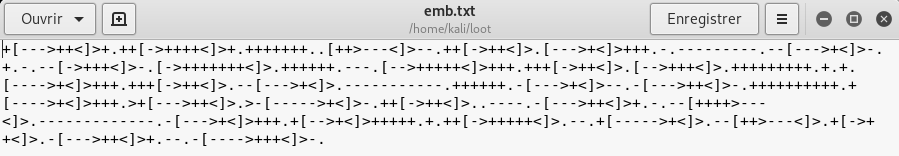
\includegraphics[width=1\textwidth]{oui/Screens/STEGHIDE/STG3.png}
  \caption{Code "Brain Fuck"}
  \label{fig:courbe-tikz}
\end{figure}

C'est un type de code original à intégrer pour rendre la capture du flag un peu plus amusante et plus complexe. \\ \\
Pour vérifier que le fichier cible aie bien incorporé le message secret, on peut taper la commande :


\begin{figure}[htp!]
  \centering
  \setlength\figureheight{7cm}
  \setlength\figurewidth{9cm}
  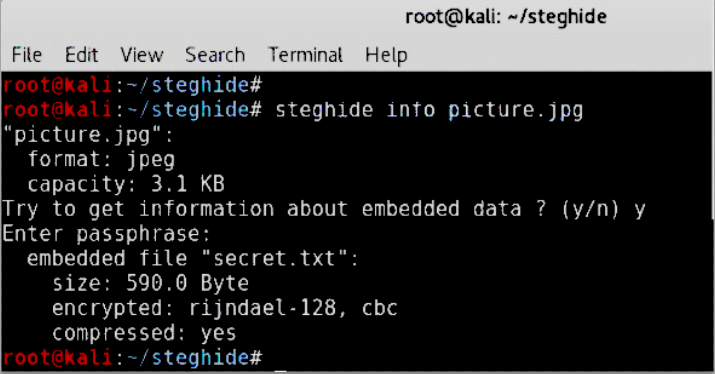
\includegraphics[width=1\textwidth]{oui/Screens/STEGHIDE/STG2.png}
  \caption{steghide info [fichier].jpeg}
  \label{fig:courbe-tikz}
\end{figure}

\newpage Comme on peut le voir, le fichier infopicture.jpg est incorporé dans un message crypté nommé secret.txt.
Maintenant, on va extraire le fichier caché avec la commande :

\begin{figure}[htp!]
  \centering
  \setlength\figureheight{7cm}
  \setlength\figurewidth{9cm}
  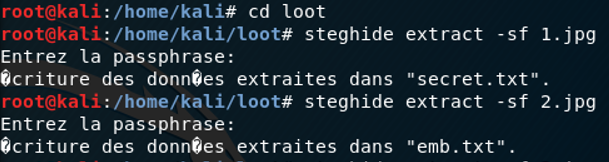
\includegraphics[width=1\textwidth]{oui/Screens/STEGHIDE/STG1.png}
  \caption{steghide extract -sf [fichier].txt}
  \label{fig:courbe-tikz}
\end{figure}

L’option -sf (--stegofile) permet de spécifier le “stego file” (fichier contenant les informations incorporées).
En affichant ensuite le contenu du fichier texte dont on a extrait le message caché, on peut donc enfin le visualiser. \\
En conclusion, cet outil simple est pratique pour récupérer des messages cachés dans des fichiers pris en charge. Cependant, son niveau d’utilisation reste assez restreint car il ne prend en charge que très peu de formats de fichiers. Cet outil est généralement utilisé en début d’attaque CTF car il a pour but de trouver des indices pour trouver les flags.
